
\chapter{Use Cases}

\section{Introduction}
Specified below are the different use cases of the application, that allows to study the interaction between user and system to achieve the functionality specified above.

\begin{figure}[h]
  \begin{center}
   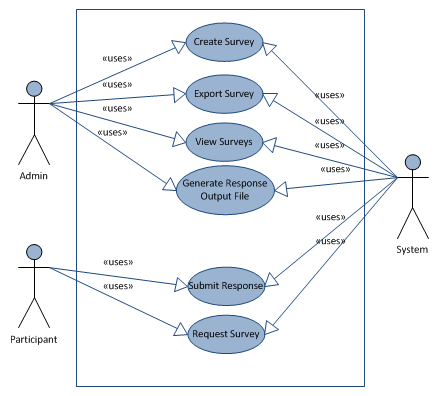
\includegraphics[width=13.3cm]{pics/usecase.png}
  \end{center}
 \caption{Use Case Diagram}
\end{figure}

\section{Use case list}
\begin{description}
\item [\ref{create}] Create Survey.
\item [\ref{manage}] Manage Surveys
\begin{description}
\item [\ref{edit}]  Edit Survey.
\item [\ref{view}] View Surveys.
\item [\ref{output}] Generate response output file.
\end{description}
\item [\ref{submit}]Submit response.
\item [\ref{request}]Request Survey.

\end{description}

\section{Use Cases}


\subsection{Create survey}
\label{create}


\begin{figure}[h!]
  \begin{center}
   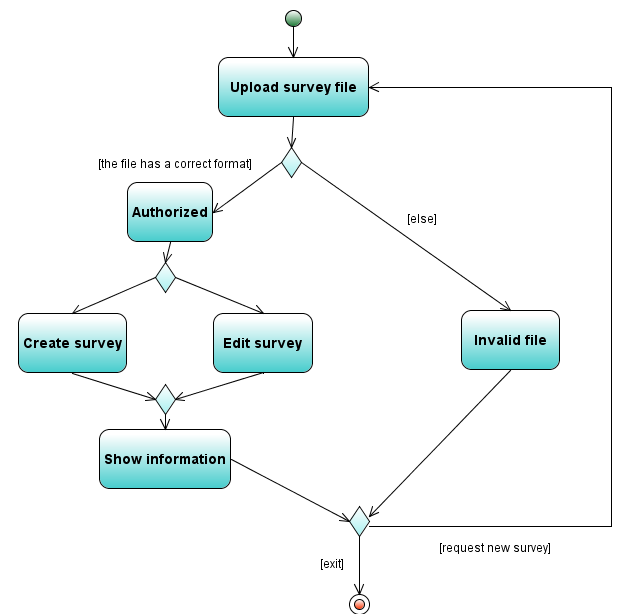
\includegraphics[width=14.6cm]{pics/Activity.png}
  \end{center}
 \caption{Activity Diagram}
\end{figure}


\setlength{\extrarowheight}{1.5mm}
\begin{tabular}{|>{\columncolor[rgb]{.3,.4,.9}}p{3.1cm} |>{\columncolor{white}} p{10.4cm} |}  \hline\hline
  \textcolor{white}{{\bf Name}} & Create Survey\\ \hline
  \textcolor{white}{{\bf Description}} & The administrator of the application creates an experiment.\\ \hline
  \textcolor{white}{{\bf Dependencies }} & None. \\ \hline
  \textcolor{white}{{\bf Actors}} & Administrator \\ \hline
  \textcolor{white}{{\bf Preconditions}} & User should have access to the system. \\  \hline
  \textcolor{white}{{\bf Postconditions}} & A new survey will be created.\\  \hline\hline
\end{tabular}


\begin{tabular}[]{|p{13.8cm}|}\hline
  \rowcolor[rgb]{.3,.4,.9}\textcolor{white}{{\bf Basic Path}} \\\hline
\end{tabular}

\begin{tabular}[]{|p{6.7cm}|p{6.7cm}|}\hline
  \rowcolor[gray]{0.9} User & System \\\hline
  1.- Access to the option Create Survey, through the main menu. & 2.- Shows an option to upload survey files. \\\hline
  3.- Select the file to upload and press OK. & 4.- Checks the validity of data. \\\hline
  & 5.- Confirms the creation of the survey.\\\hline
\end{tabular}\\ 

\begin{tabular}[]{|p{13.8cm}|}\hline
  \rowcolor[rgb]{.3,.4,.9}\textcolor{white}{{\bf Alternative Paths }} \\\hline
\end{tabular}\\ 

\begin{tabular}[]{|p{6.7cm}|p{6.7cm}|}\hline
  \rowcolor[gray]{0.9} User & System \\\hline
  & 5b.- The data is incorrect. Asks for another file input. \\\hline
\end{tabular}

\begin{figure}[h!]
  \begin{center}
   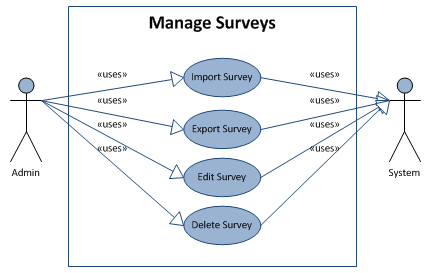
\includegraphics[width=13.6cm]{pics/ManageSurveys.png}
  \end{center}
 \caption{Use Case Diagram}
\end{figure}

\subsection{Manage Surveys}
\label{manage}

\begin{figure}[h!]
  \begin{center}
   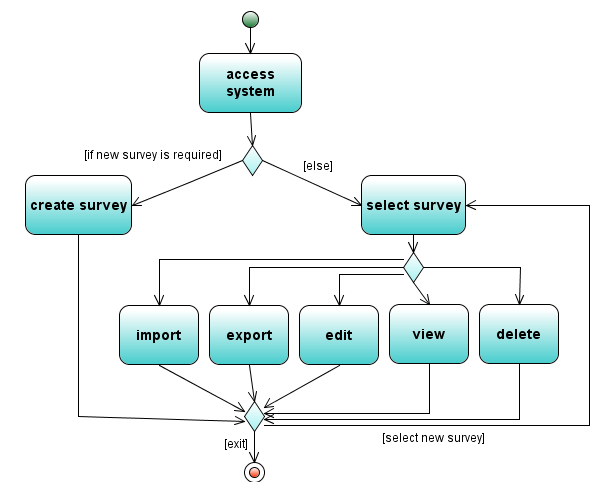
\includegraphics[width=13.3cm]{pics/Activity2.png}
  \end{center}
 \caption{Activity Diagram}
\end{figure}
\subsubsection{ Edit survey}
\label{edit}

\setlength{\extrarowheight}{1.5mm}
\begin{tabular}{|>{\columncolor[rgb]{.3,.4,.9}}p{3.1cm} |>{\columncolor{white}} p{10.4cm} |}  \hline\hline
  \textcolor{white}{{\bf Name}} & Edit Survey\\ \hline
  \textcolor{white}{{\bf Description}} & The user edits an existing survey. \\ \hline
  \textcolor{white}{{\bf Dependencies }} & \ref{create}  \\ \hline
  \textcolor{white}{{\bf Actors}} & Administrator \\ \hline
  \textcolor{white}{{\bf Preconditions}} & A survey must have been already created. \\ \hline
  \textcolor{white}{{\bf Postconditions}} & An existing survey will be changed.\\ \hline\hline
\end{tabular}


\begin{tabular}{|p{13.8cm}|}\hline
  \rowcolor[rgb]{.3,.4,.9}\textcolor{white}{{\bf Basic Path}} \\\hline
\end{tabular}

\begin{tabular}[]{|p{6.7cm}|p{6.7cm}|}\hline
  \rowcolor[gray]{0.9} User & System \\\hline
  1.- Choose the option {\it Edit survey} in the menu. & 2.- Shows the options for editing the file. \\\hline
  3.- Chage the options and  press OK. & 4.- Checks validity of data. \\\hline
  & 5.- Confirms the edition of the survey.\\\hline
\end{tabular}\\ 

\begin{tabular}[]{|p{13.8cm}|}\hline
  \rowcolor[rgb]{.3,.4,.9}\textcolor{white}{{\bf Alternative Paths }} \\\hline
\end{tabular}\\ 

\begin{tabular}[]{|p{6.7cm}|p{6.7cm}|}\hline
  \rowcolor[gray]{0.9} User & System \\\hline
  & 5b.- The data is incorrect. Returns to step 2.\\\hline
\end{tabular}

\subsubsection{ View Surveys}
\label{view}

\setlength{\extrarowheight}{1.5mm}
\begin{tabular}{|>{\columncolor[rgb]{.3,.4,.9}}p{3.1cm} |>{\columncolor{white}} p{10.4cm} |}  \hline\hline
  \textcolor{white}{{\bf Name}} & View Surveys\\ \hline
  \textcolor{white}{{\bf Description}} & The user views the existing surveys.\\ \hline
  \textcolor{white}{{\bf Dependencies }} & \ref{create}  \\ \hline
  \textcolor{white}{{\bf Actors}} & Administrator \\ \hline
  \textcolor{white}{{\bf Preconditions}} & The user must have access to the system. \\\hline
  \textcolor{white}{{\bf Postconditions}} & The survey(s) will be displayed on the screen.\\\hline\hline
\end{tabular}


\begin{tabular}{|p{13.8cm}|}\hline
  \rowcolor[rgb]{.3,.4,.9}\textcolor{white}{{\bf Basic Path}} \\\hline
\end{tabular}

\begin{tabular}[]{|p{6.7cm}|p{6.7cm}|}\hline
  \rowcolor[gray]{0.9} User & System \\\hline
  1.- Choose the option {\it View surveys}. & 2.- Displays a menu, with all the current surveys in the system. \\\hline
  3.- Choose a survey within the given list. & 4.- Shows the selected survey. \\\hline
\end{tabular}\\ 

\begin{tabular}[]{|p{13.8cm}|}\hline
  \rowcolor[rgb]{.3,.4,.9}\textcolor{white}{{\bf Alternative Paths }} \\\hline
\end{tabular}\\ 

\begin{tabular}[]{|p{6.7cm}|p{6.7cm}|}\hline
  \rowcolor[gray]{0.9} User & System \\\hline
  & 2b.- There are no surveys in the system. Displays the message: {\it There are no surveys available.} \\\hline
  & 4b.- If the systems fails while accessing the required data, it returns to step 2.   \\\hline
\end{tabular}

\subsection{ Generate Response Output File}
\label{output}

\setlength{\extrarowheight}{1.5mm}
\begin{tabular}{|>{\columncolor[rgb]{.3,.4,.9}}p{3.1cm} |>{\columncolor{white}} p{10.4cm} |}  \hline\hline
  \textcolor{white}{{\bf Name}} & Generate response output file.\\ \hline
  \textcolor{white}{{\bf Description}} & Generates an output file containing all surveys responses. \\\hline
  \textcolor{white}{{\bf Dependencies }} & \ref{create}  \ref{submit}\\ \hline
  \textcolor{white}{{\bf Actors}} & Administrator \\ \hline
  \textcolor{white}{{\bf Preconditions}} & A survey must have been already created and submited. \\ \hline
  \textcolor{white}{{\bf Postconditions}} & An output file will be created.\\ \hline\hline
\end{tabular}


\begin{tabular}{|p{13.8cm}|}\hline
  \rowcolor[rgb]{.3,.4,.9}\textcolor{white}{{\bf Basic Path}} \\\hline
\end{tabular}

\begin{tabular}[]{|p{6.7cm}|p{6.7cm}|}\hline
  \rowcolor[gray]{0.9} User & System \\\hline
  1.- Choose the option {\it Generate Response File}. & 2.- Shows a list with all the current surveys. \\\hline
  3.- Selects a survey from which to obtain the output file and selects Ok. & 4.- Displays a window with Saving options. \\\hline
  5.- Selects a path where to store the output file, and a name for the file. Clicks {\it Save} & 6.- Performs the operation and displays an operation completed message.\\\hline
\end{tabular}\\ 

\begin{tabular}[]{|p{13.8cm}|}\hline
  \rowcolor[rgb]{.3,.4,.9}\textcolor{white}{{\bf Alternative Paths }} \\\hline
\end{tabular}\\ 

\begin{tabular}[]{|p{6.7cm}|p{6.7cm}|}\hline
  \rowcolor[gray]{0.9} User & System \\\hline
  & 6b.- The operation could not be done. No file was generated. Returns to step 2. \\\hline
\end{tabular}

\subsection{Request Survey }
\label{request}

\begin{figure}[h!]
  \begin{center}
   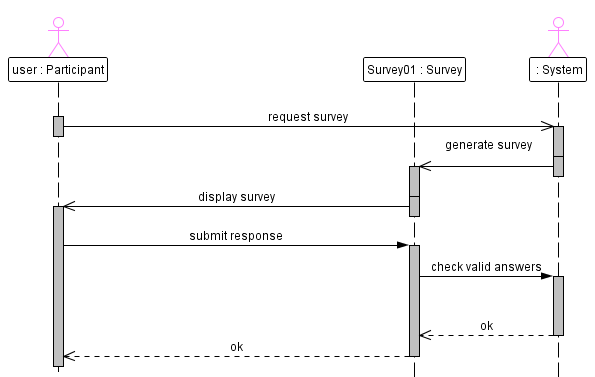
\includegraphics[width=15cm]{pics/Sequence.png}
  \end{center}
 \caption{Sequence Diagram}
\end{figure}

\setlength{\extrarowheight}{1.5mm}
\begin{tabular}{|>{\columncolor[rgb]{.3,.4,.9}}p{3.1cm} |>{\columncolor{white}} p{10.4cm} |}  \hline\hline
  \textcolor{white}{{\bf Name}} & Request Survey\\\hline
  \textcolor{white}{{\bf Description}} & The user request a new survey to be displayed. \\\hline
  \textcolor{white}{{\bf Dependencies }} & \ref{create}  \\\hline
  \textcolor{white}{{\bf Actors}} & Participant \\ \hline
  \textcolor{white}{{\bf Preconditions}} & A survey must have been already created. \\ \hline
  \textcolor{white}{{\bf Postconditions}} & A survey will be displayed.\\ \hline\hline
\end{tabular}


\begin{tabular}{|p{13.8cm}|}\hline
  \rowcolor[rgb]{.3,.4,.9}\textcolor{white}{{\bf Basic Path}} \\\hline
\end{tabular}

\begin{tabular}[]{|p{6.7cm}|p{6.7cm}|}\hline
  \rowcolor[gray]{0.9} User & System \\\hline
  1.- Enters the URL in the web browser. & 2.- Shows the main menu to the user. \\\hline
  3.- Selects the option {\it Request Survey}. & 4.- Presents a list of surveys . \\\hline
  4.- Chooses a survey. & 6.- Displays a version of the selected survey.\\\hline
\end{tabular}\\ 

\begin{tabular}[]{|p{13.8cm}|}\hline
  \rowcolor[rgb]{.3,.4,.9}\textcolor{white}{{\bf Alternative Paths }} \\\hline
\end{tabular}\\ 

\begin{tabular}[]{|p{6.7cm}|p{6.7cm}|}\hline
  \rowcolor[gray]{0.9} User & System \\\hline
  &  \\\hline
\end{tabular}

\subsection{ Submit Response}
\label{submit}

\setlength{\extrarowheight}{1.5mm}
\begin{tabular}{|>{\columncolor[rgb]{.3,.4,.9}}p{3.1cm} |>{\columncolor{white}} p{10.4cm} |}  \hline\hline
  \textcolor{white}{{\bf Name}} & Submit Response\\ \hline
  \textcolor{white}{{\bf Description}} & The user submits a fully completed survey. \\\hline
  \textcolor{white}{{\bf Dependencies }} & \ref{request}  \\\hline
  \textcolor{white}{{\bf Actors}} & Participant \\\hline
  \textcolor{white}{{\bf Preconditions}} & A survey must have been already requested. \\\hline
  \textcolor{white}{{\bf Postconditions}} & A survey response will be submitted.\\\hline\hline
\end{tabular}


\begin{tabular}{|p{13.8cm}|}\hline
  \rowcolor[rgb]{.3,.4,.9}\textcolor{white}{{\bf Basic Path}} \\\hline
\end{tabular}

\begin{tabular}[]{|p{6.7cm}|p{6.7cm}|}\hline
  \rowcolor[gray]{0.9} User & System \\\hline
  1.- Choose the option {\it Submit Survey}. & 2.- Stores the data and Shows a congratulations message. \\\hline
\end{tabular}\\ 

\begin{tabular}[]{|p{13.8cm}|}\hline
  \rowcolor[rgb]{.3,.4,.9}\textcolor{white}{{\bf Alternative Paths }} \\\hline
\end{tabular}\\ 

\begin{tabular}[]{|p{6.7cm}|p{6.7cm}|}\hline
  \rowcolor[gray]{0.9} User & System \\\hline
  &  2b.- If there are any incomplete box, shows the survey again.  \\\hline
\end{tabular}

